\section*{Abstract}
		Diese Übersicht präsentiert die vollständige T0-Theorieserie bestehend aus 8 fundamentalen Dokumenten, die eine geometrische Reformulierung der Physik darstellen. Basierend auf einem einzigen Parameter $\xi = \frac{4}{3} \times 10^{-4}$, zusammen mit festen rationalen Strukturwahlen, werden fundamentale Konstanten, Teilchenmassen und physikalische Phänomene von der Quantenmechanik bis zur Kosmologie in einem Rahmen beschrieben; SI-Anker wie $E_0$, $m_e$ oder $v$ dienen der Umrechnung, nicht der Ableitung. Viele Werte werden auf rund 1\,\% getroffen; weil die Leiterparameter $r_i$, $p_i$ gesetzt sind und ein Anker den Anschluss an das SI leistet, sind diese Übereinstimmungen keine unabhängigen Belege. Den kosmischen Sektor ($H_0$, $\Lambda$, Dunkle Energie) klammert die Serie bewusst aus, weil auch das Standardmodell ihn nicht herleitet; die kosmologischen Aussagen sind spekulativ. Die Theorie bietet testbare Vorhersagen für zukünftige Experimente.

	

	\section{Dokumentenserie: Systematischer Aufbau}
	
	\subsection{Hierarchische Struktur der 8 Dokumente}
	
	Die T0-Dokumentenserie folgt einer logischen Progression von fundamentalen Prinzipien zu spezifischen Anwendungen:
	
	\begin{center}
		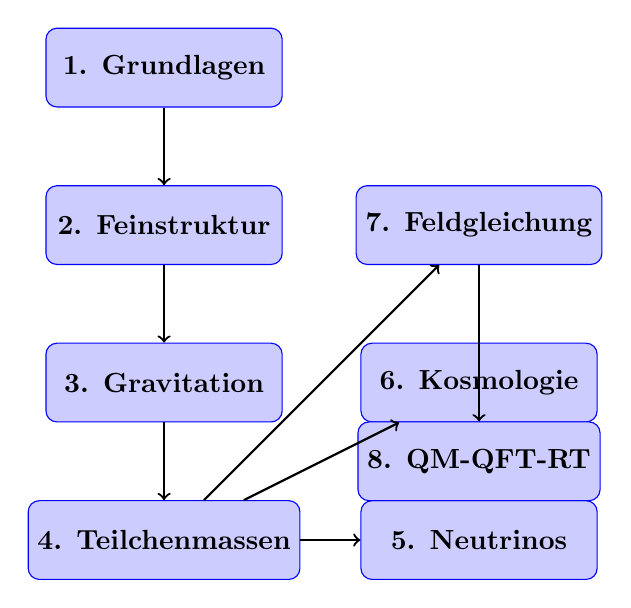
\begin{tikzpicture}[node distance=2cm]
			\tikzstyle{doc} = [rectangle, rounded corners, minimum width=3cm, minimum height=1cm, text centered, draw=blue, fill=blue!20]
			\tikzstyle{arrow} = [thick,->]
			
			\node [doc] (doc1) {\textbf{1. Grundlagen}};
			\node [doc, below of=doc1] (doc2) {\textbf{2. Feinstruktur}};
			\node [doc, below of=doc2] (doc3) {\textbf{3. Gravitation}};
			\node [doc, below of=doc3] (doc4) {\textbf{4. Teilchenmassen}};
			\node [doc, right of=doc4, xshift=2cm] (doc5) {\textbf{5. Neutrinos}};
			\node [doc, above of=doc5] (doc6) {\textbf{6. Kosmologie}};
			\node [doc, above of=doc6] (doc7) {\textbf{7. Feldgleichung}};
			\node [doc, below of=doc7, yshift=-1cm] (doc8) {\textbf{8. QM-QFT-RT}};
			
			\draw [arrow] (doc1) -- (doc2);
			\draw [arrow] (doc2) -- (doc3);
			\draw [arrow] (doc3) -- (doc4);
			\draw [arrow] (doc4) -- (doc5);
			\draw [arrow] (doc4) -- (doc6);
			\draw [arrow] (doc4) -- (doc7);
			\draw [arrow] (doc7) -- (doc8);
		\end{tikzpicture}
	\end{center}
	
	\section{Dokument 1: 003\_T0\_Grundlagen\_v1\_De.pdf}
	
	\begin{documentbox}
		\textbf{Untertitel:} Die geometrischen Grundlagen der Physik
		
		\textbf{Zentrale Inhalte:}
		\begin{itemize}
			\item \textbf{Fundamentaler Parameter:} $\xi = \frac{4}{3} \times 10^{-4}$ als geometrische Konstante
			\item \textbf{Zeit-Masse-Dualität:} $T \cdot m = 1$ in natürlichen Einheiten
			\item \textbf{Fraktale Raumzeitstruktur:} $D_f^{\text{eff}} \approx 2{,}973$ und $K_{\text{frak}} \approx 0{,}987$
			\item \textbf{Interpretationsebenen:} Harmonisch, geometrisch, feldtheoretisch
			\item \textbf{Universelle Formelstruktur:} Template für alle T0-Beziehungen
		\end{itemize}
		
		\textbf{Fundamentale Erkenntnisse:}
		\begin{itemize}
			\item Tetraedrische Packung als Raumgrundstruktur
			\item Quantenfeldtheoretische Herleitung von $10^{-4}$
			\item Charakteristische Energieskalen: $E_0 = 7.398$ MeV
			\item Philosophische Implikationen der geometrischen Physik
		\end{itemize}
		
		\textbf{Status:} Theoretische Grundlage - vollständig etabliert
	\end{documentbox}
	
	\section{Dokument 2: 011\_T0\_Feinstruktur\_De.pdf}
	
	\begin{documentbox}
		\textbf{Untertitel:} Herleitung von $\alpha$ aus geometrischen Prinzipien
		
		\textbf{Zentrale Formel:}
		\begin{equation}
			\boxed{\alpha = \xi \cdot \left(\frac{E_0}{1\,\text{MeV}}\right)^2}
		\end{equation}
		
		\textbf{Schlüsselergebnisse:}
		\begin{itemize}
			\item \textbf{T0-Wert:} $\alpha^{-1} = 137.04$
			\item \textbf{Experiment:} $\alpha^{-1} = 137.036$
			\item \textbf{Abweichung:} 0.003\%
			\item \textbf{Einordnung:} Die Übereinstimmung ist eine Eigenschaft des Ankers $E_0$, der den einzigen Anschluss an das SI leistet; sie ist keine unabhängige Vorhersage.
		\end{itemize}
		
		\textbf{Theoretische Innovationen:}
		\begin{itemize}
			\item Charakteristische Energie $E_0 = \sqrt{m_e \cdot m_\mu/K_{\text{frak}}}$ (nackt $\sqrt{m_e m_\mu}$, R72)
			\item Logarithmische Symmetrie der Leptonmassen
			\item Fundamentale Abhängigkeit $\alpha = \xi E_0^2$ mit $E_0 = \sqrt{m_e m_\mu/K_{\text{frak}}}$
			\item Warum Zahlenverhältnisse nicht gekürzt werden dürfen
		\end{itemize}
		
		\textbf{Status:} $\alpha = \xi E_0^2$ als Beziehung über den Anker $E_0$
	\end{documentbox}
	
	\section{Dokument 3: 012\_T0\_Gravitationskonstante\_De.pdf}
	
	\begin{documentbox}
		\textbf{Untertitel:} Systematische Herleitung von $G$ aus geometrischen Prinzipien
		
		\textbf{Vollständige Formel:}
		\begin{equation}
			\boxed{G_{\text{SI}} = \frac{\xi^2}{4 m_e} \times C_{\text{conv}} \times K_{\text{frak}}}
		\end{equation}
		
		\textbf{Umrechnungsfaktoren:}
		\begin{itemize}
			\item \textbf{Dimensionskorrektur:} $C_1 = 1/E_{\text{char}} = 3.472 \times 10^{-2}$ mit $E_{\text{char}} = 28.8$ (Dok.~012); $C_1$ kommt in der Boxformel oben nicht vor, diese gilt ohne $C_1$
			\item \textbf{SI-Konversion:} $C_{\text{conv}} = 7.783 \times 10^{-3}$
			\item \textbf{Fraktale Korrektur:} $K_{\text{frak}} = 0.986$
		\end{itemize}
		
		\textbf{Experimentelle Verifikation:}
		\begin{itemize}
			\item \textbf{T0-Vorhersage:} $G = 6.6745 \times 10^{-11}$ m³/(kg·s²)
			\item \textbf{CODATA 2018:} $G = 6.67430 \times 10^{-11}$ m³/(kg·s²)
			\item \textbf{Abweichung:} +0.003\%
		\end{itemize}
		
		Die Boxformel mit den angegebenen Faktoren ergibt $6.6745\times10^{-11}$. $C_{\text{conv}}$ ist die SI-Umrechnung der Ein-Anker-Kette (Dok.~383); ihr Zahlenwert $7.783\times10^{-3}$ enthält zusätzlich den kleinen Rest dieser Kette (Kettenwert $7.58\times10^{-3}$). Die Form von $G$ und seine Größenordnung folgen aus $\xi$ und dem einen Anker (in Dok.~383 numerisch geprüft); mit dem Anker $m_e$ liegt $G$ bei $-2.6\,\%$, mit $v$ bei $-0.46\,\%$. Die Übereinstimmung auf $0.003\,\%$ ergibt sich erst mit diesem Rest und gilt nicht als eigener Präzisionsbeleg.
		
		\textbf{Physikalische Bedeutung:} Gravitation als geometrische Raumzeit-Materie-Kopplung
		
		\textbf{Status:} Form und Größenordnung aus $\xi$ und einem Anker; die CODATA-Übereinstimmung ist kein eigener Präzisionsbeleg
	\end{documentbox}
	
	\section{Dokument 4: 006\_T0\_Teilchenmassen\_De.pdf}
	
	\begin{documentbox}
		\textbf{Untertitel:} Fermionmassen aus der Leiter $m_i = r_i\,\xi^{p_i}\,v$
		
		\textbf{Zwei äquivalente Methoden:}
		\begin{enumerate}
			\item \textbf{Direkte Methode:} $m_i = 1/(\xi f_i)$, über $f_i = 1/(r_i\,\xi^{p_i+1}\,v)$ mit der Yukawa-Methode verknüpft; die Übereinstimmung beider Methoden gilt per Konstruktion
			\item \textbf{Erweiterte Yukawa:} $m_i = y_i \times v$ mit $y_i = r_i \times \xi^{p_i}$
		\end{enumerate}
		
		\textbf{Quantenzahlen-System:} Rationale Quantenzahlen $(r_i, p_i)$ als feste Strukturwahlen; $v$ dient als Umrechnungsanker
		
		\textbf{Vergleich mit dem Experiment:} Für geladene Leptonen und Quarks liegt die durchschnittliche Abweichung unter 1\,\%. Weil $r_i$ und $p_i$ gesetzt und an die Messwerte angepasst sind, sind diese Übereinstimmungen Identitäten der Leiter und keine eigenen Belege; die Massenverhältnisse folgen aus der Leiter auf wenige Stellen. Neutrinomassen werden in Dok.~006 nicht berechnet (maßgeblich Dok.~340), Bosonenmassen behandeln Dok.~372 und~373.
		
		\textbf{Reduktion:} Die freien Massenparameter des Standardmodells werden auf $\xi$ und die gesetzten rationalen Quantenzahlen $(r_i, p_i)$ zurückgeführt; es bleibt kein kontinuierlich einstellbarer Parameter.
		
		\textbf{Status:} Leiterstruktur mit gesetzten Quantenzahlen und einem Anker
	\end{documentbox}
	
	\section{Dokument 5: 007\_T0\_Neutrinos\_De.pdf}
	
	\begin{documentbox}
		\textbf{Untertitel:} Die Photon-Analogie und geometrische Oszillationen
		
		\textbf{Ansatz:}
		\begin{itemize}
			\item \textbf{Photon-Analogie:} Neutrinos als ''gedämpfte Photonen''
			\item \textbf{Doppelte $\xi$-Suppression:} Basiswert $m_\nu = \frac{\xi^2}{2} \times m_e = 4.54$ meV
			\item \textbf{Geometrische Oszillationen:} Phasen statt Massendifferenzen
		\end{itemize}
		
		\textbf{Experimentelle Einordnung:}
		\begin{itemize}
			\item \textbf{Spektrum:} Ein für alle Flavors (nahezu) einheitliches Spektrum mit $\Sigma m_\nu \approx 13.6$ meV ist ausgeschlossen, weil die gemessenen Massendifferenzen $\Sigma m_\nu \geq 59$ meV verlangen.
			\item \textbf{Geschwindigkeit:} Eine energieunabhängige Differenz $v_\nu = c(1 - \xi^2/2)$ gilt nicht, weil $\xi^2/2$ das Massenverhältnis $m_\nu/m_e$ ist.
			\item \textbf{Maßgeblich:} Für Neutrinos ist Dok.~340 maßgeblich; dort tritt der Basiswert $4.54$ meV als leichteste Masse $m_{\nu_1}$ wieder auf.
		\end{itemize}
		
		\textbf{Status:} Spekulativ; das Spektrum von Dok.~007 ist durch die Oszillationsdaten ausgeschlossen, maßgeblich ist Dok.~340
	\end{documentbox}
	
	\section{Dokument 6: 025\_T0\_Kosmologie\_De.pdf}
	
	\begin{documentbox}
		\textbf{Untertitel:} Statisches Universum und $\xi$-Feld-Manifestationen
		
		\textbf{Kosmologie:}
		\begin{itemize}
			\item \textbf{Statisches Universum:} Kein Urknall, ewig existierend
			\item \textbf{Zeit-Energie-Dualität:} Kein singulärer Anfang, weil $T\cdot E = 1$ mit der unteren Zeitschranke $T_0 = \xi\,t_P$ die Energie nach oben beschränkt und der Torus keinen Rand hat (Dok.~306)
			\item \textbf{CMB aus $\xi$-Feld:} Nicht aus z=1100-Entkopplung
		\end{itemize}
		
		\textbf{Casimir-CMB-Verbindung:}
		\begin{itemize}
			\item \textbf{Charakteristische Länge:} $L_\xi = 100$ $\mu$m
			\item \textbf{Verhältnis bei $L_\xi$:} $|\rho_{\text{Casimir}}|/\rho_{\text{CMB}} = 308$ -- eine Identität, kein Messbeleg, weil $L_\xi$ selbst aus der gemessenen CMB-Energiedichte und $\xi$ bestimmt wird; ein Vergleichswert $312$ ist dieselbe Formel mit gerundetem $L_\xi$. Die Verbindung ist eine Skalenaussage (spekulativ).
			\item \textbf{Vertiefung:} Dok.~279 -- Casimir-CMB-H$_0$-Verbindungsformel, $L_\xi H_0/c = K_{\text{geo}}\,(m_e c^2/k_B T_{\text{CMB}})\,\xi^{41/4}$.
		\end{itemize}
		
		\textbf{Alternative Rotverschiebung (statisch, achromatisch):}
		\begin{equation}
			1+z = e^{\xi x}, \qquad z \approx \xi \cdot x
		\end{equation}
		Die fraktale Wegverlängerung ist rein geometrisch und streckt alle
		Wellenlängen um denselben Faktor; die Rotverschiebung ist \emph{achromatisch}
		(Finite-Elemente-Simulation). Die Längenskala von $x$ folgt nicht aus $\xi$
		allein, sondern ist über den gemessenen $H_0$ kalibriert. Vertiefung: Dok.~280 (z$\to$Zeit als $\Lambda$CDM-Übertragung, kosmologische
		Entartung Dok.~267, $z_*\approx 875$ als T$^4$-Gitterresonanz).
		
		\textbf{Kosmologische Probleme (spekulativ):}
		\begin{itemize}
			\item Horizontproblem, Flachheitsproblem, Monopolproblem, Altersproblem
			\item $H_0$ und $\Lambda$ folgen nicht aus $\xi$ allein: Die Skala der Rotverschiebung ist über den gemessenen $H_0$ kalibriert. Hubble-Spannung und Dunkle Energie gelten daher nicht als gelöst; der kosmische Sektor ist bewusst ausgeklammert, weil auch das Standardmodell ihn nicht herleitet.
		\end{itemize}
		
		\textbf{Status:} Testbare Hypothesen - spekulative Alternative, kosmischer Sektor kalibriert
	\end{documentbox}
	
	\section{Dokument 7: T0\_Feldgleichung\_De.pdf}
	
	\begin{documentbox}
		\textbf{Untertitel:} Die fundamentale Feldgleichung der T0-Theorie
		
		\textbf{Zentrale Inhalte:}
		\begin{itemize}
			\item \textbf{Fundamentale Feldgleichung:} $\square \Phi + \xi \cdot \mathcal{F}[\Phi] = 0$
			\item \textbf{Geometrische Interpretation:} Feld als Manifestation der Raumstruktur
			\item \textbf{Vereinheitlichung:} Alle Wechselwirkungen aus einer Gleichung
			\item \textbf{Lösungsklassen:} Teilchenlösungen, Wellenlösungen, Vakuumlösungen
		\end{itemize}
		
		\textbf{Physikalische Konsequenzen:}
		\begin{itemize}
			\item Emergente Eichsymmetrien aus geometrischen Einschränkungen
			\item Quantisierung als natürliche Konsequenz der Feldgeometrie
			\item Skalenstruktur aus der Rekursion $\mathcal{R}$ (kein RG-Verfahren)
			\item Phasenübergänge als topologische Veränderungen
		\end{itemize}
		
		\textbf{Status:} Theoretischer Rahmen - vollständig formuliert
	\end{documentbox}
	
	\section{Dokument 8: 020\_T0\_QM-QFT-RT\_De.pdf}
	
	\begin{documentbox}
		\textbf{Untertitel:} Vereinheitlichung von QM, QFT und RT aus einer geometrischen Grundlage
		
		\textbf{Zentrale Inhalte:}
		\begin{itemize}
			\item \textbf{Universelle T0-Feldgleichung:} $\square \Phi + \xi \cdot \mathcal{F}[\Phi] = 0$ als Grundlage aller Theorien
			\item \textbf{Zeit-Masse-Dualität:} $T \cdot m = 1$ verbindet alle drei Säulen der Physik
			\item \textbf{Emergente Quanteneigenschaften:} QM als Approximation des Energiefeldes
			\item \textbf{Feldbeschreibung:} Alle Teilchen als Anregungen eines fundamentalen Feldes $\Phi$
			\item \textbf{Renormierungslösung:} Natürlicher Cutoff durch $E_P/\xi$
					\end{itemize}
		
		\textbf{Fundamentale Erkenntnisse:}
		\begin{itemize}
			\item Deterministische Deutung der Quantenmechanik über das Zeitfeld (spekulativ; lokal nur unter der Annahme des Superdeterminismus, die Bell-Verletzung bleibt)
			\item Welle-Teilchen-Dualität aus Feldgeometrie
			\item Energieskalen-Hierarchie: Planck bis QCD durch $\xi$-Korrekturen
			\item Gravitation als Feldkrümmung
			\item Philosophische Implikationen: Einheit der Physik durch geometrische Prinzipien
		\end{itemize}
		
		\textbf{Status:} Theoretische Vereinheitlichung - baut auf allen vorherigen Dokumenten auf, testbare Vorhersagen
	\end{documentbox}

	\section{Vergleichs- und Einordnungsserie (IPI-Feld)}

	Ergänzend zur Grundlagen-Serie oben dokumentiert eine eigene Reihe die Stellung der
	FFGFT gegenüber anderen im Information-Physics-Institute diskutierten Rahmenwerken.
	Diese Dokumente sind \emph{Vergleiche und Einordnungen}, keine neuen Grundlagen:
	\begin{itemize}
		\item \textbf{Dok.~245} -- FFGFT abgebildet auf RA~2.1 (Guevara).
		\item \textbf{Dok.~246} -- FFGFT vs.\ RSG (Austin): asymmetrische Komplementarität.
		\item \textbf{Dok.~251} -- FFGFT vs.\ Vopson (MEI / Computational Universe): geometrie- vs.\ informations-primitiv.
		\item \textbf{Dok.~260} -- FFGFT vs.\ UC (Haskins): Constraint, $\alpha$-Korrektur-Inkonsistenz.
		\item \textbf{Dok.~269} -- FFGFT $\leftrightarrow$ RA/PMT (Guevara), bidirektional.
		\item \textbf{Dok.~271} -- FFGFT $\leftrightarrow$ HLV (Krüger), paarweiser Vergleich; spektrale Gabel.
		\item \textbf{Dok.~272} -- FFGFT $\leftrightarrow$ HLV über die Dot-Governance-Schicht (Vossen).
		\item \textbf{Dok.~274} -- FFGFT im IPI-Feld: Substrat- und Primitiv-Achsen (Landkarte); A*-Worked-Example.
	\end{itemize}
	\textbf{Status:} laufende Korrespondenz-Serie, datiert und vorläufig; jede Einordnung ist eine
	erklärte Lesart (O2), das primäre Rendering (O0) verbleibt beim jeweiligen Urheber.
